\documentclass[12pt]{article}
\usepackage[french]{babel}
\usepackage[utf8]{inputenc}
\usepackage[ruled,vlined]{algorithm2e}
\usepackage{amsmath}
\usepackage{amssymb}
\usepackage{csquotes}
\usepackage[T1]{fontenc} 
\usepackage{listings}
\lstset { %
    language=C++, % set backgroundcolor
    basicstyle=\footnotesize,% basic font setting
}
\newcommand{\mycode}{                               % Name after the Language used
    \lstset{
        basicstyle=\ttfamily\small,                 % Code Font Size
        keywordstyle=\color{darkpurple}\bfseries,   % Color Key Word
        stringstyle=\color{darkblue},               % Color String
        identifierstyle=\color{teal},
        commentstyle=\color{darkgreen},             % Color Comment
        morecomment=[s][\color{blue}]{/**}{*/},     % Color Comment
        tabsize=2,                                  % Tab Size
        captionpos=b,                               % Caption Position
        showtabs=false,                             % Show Tabs within Strings
        showspaces=false,                           % Show Spaces Code
        showstringspaces=false,                     % Show Spaces Strings
        stepnumber=1,                               % Line Number Step
        numbers=left,                               % Line Number Position
        numbersep=5pt,                              % Line Number Distance from Code
        numberstyle=\tiny\color{gray},              % Line Number Style
        frame=single,                               % Frame
        rulecolor=\color{black},                    % Frame Color
        xleftmargin=10pt,                            % Left Margin
        backgroundcolor=\color{white},              % Background Color
        breaklines=true,                            % Break Automatic Line
        breakatwhitespace=true,                     % Break Automatic Spaces 
        breakautoindent=false,                      % Break Automatic Indent
        extendedchars=true,                         % 
        inputencoding=latin1,                       % Encoding
        literate=                                   % Including Especial Charects
                {é}{{\'{e}}}1
                {è}{{\`{e}}}1
                {ê}{{\^{e}}}1
                {ë}{{\¨{e}}}1
                {É}{{\'{E}}}1
                {Ê}{{\^{E}}}1
                {û}{{\^{u}}}1
                {ù}{{\`{u}}}1
                {ú}{{\'{u}}}1
                {â}{{\^{a}}}1
                {à}{{\`{a}}}1
                {á}{{\'{a}}}1
                {ã}{{\~{a}}}1
                {ä}{{\"{a}}}1
                {Á}{{\'{A}}}1
                {Â}{{\^{A}}}1
                {Ã}{{\~{A}}}1
                {Ä}{{\"{A}}}1
                {ç}{{\c{c}}}1
                {Ç}{{\c{C}}}1
                {õ}{{\~{o}}}1
                {ó}{{\'{o}}}1
                {ô}{{\^{o}}}1
                {ö}{{\"{o}}}1
                {Õ}{{\~{O}}}1
                {Ó}{{\'{O}}}1
                {Ô}{{\^{O}}}1
                {Ö}{{\"{O}}}1
                {î}{{\^{i}}}1
                {Î}{{\^{I}}}1
                {í}{{\'{i}}}1
                {Í}{{\~{Í}}}1
                {ü}{{\"{u}}}1
                {Ü}{{\"{U}}}1
    }
}



\usepackage{geometry}
 \geometry{
 a4paper,
 total={170mm,257mm},
 left=20mm,
 top=20mm,
 }
\usepackage{float}
\usepackage{graphicx}
\graphicspath{ {./images/} }
\usepackage{wrapfig}

\usepackage{graphicx}
\usepackage{color}

\sloppy
\definecolor{lightgray}{gray}{0.5}
% \setlength{\parindent}{0pt}

\usepackage{caption}
\usepackage{subcaption}
\usepackage{tabularray}
\usepackage{hyperref}

\usepackage[backend=biber, sorting=ynt]{biblatex}
\addbibresource{refs.bib}








\begin{document}
% \setlength{\parindent}{0pt}

\begin{titlepage}
 \centering
 \vspace*{1in}
 \begin{figure}[t]
    \centering
    
\includegraphics[scale=0.5]{images/Logo_ENSTA_Paris.jpg}
\end{figure}
 \begin{Huge}\bfseries
 IA301 - Logics and Symbolic AI
  
  TP\par
 \end{Huge}
 \vspace{1.5in}
 \begin{large}\bfseries

  
Joaquim Minarelli Gaspar\\
Filipe Lacerda\\
Eduardo Guimarães\\
Yaël Gossec

 \end{large}
 \vfill
	 
 
 \vspace{0.5in}
 Palaiseau, France
 \par
 
 \vspace{0.5in}
 Novembre 2024
 \par
\end{titlepage}

\tableofcontents

\newpage

\section{OWL with Protege}
\subsection{Simple Ontology (Preliminary Case)}

We explored the tool using the given example. The results are presented below.
\\

\smallskip
\begin{itemize}
    \item What do we observe when we check the inferred classes ?
\end{itemize}
\smallskip
Answer :    The inferred classes are the same as the asserted classes. This means that there are no additional logical consequences or inferences made by the reasoner beyond what has already been explicitly asserted in the ontology. This indicates that the ontology is consistent, and the asserted hierarchy or relationships between classes are correctly modeled according to the ontology's logical structure.

\begin{itemize}
    \item Some DL queries examples and results.
\end{itemize}

\begin{figure}[H]
    \centering
    \begin{minipage}[b]{0.25\textwidth}
        \centering
        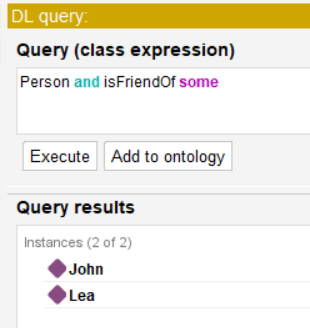
\includegraphics[width=\textwidth]{images/1.1 - tuto/DL query.png}
        \caption{Persons who have friends}
        \label{fig:image1}
    \end{minipage}
    \hfill
    \begin{minipage}[b]{0.25\textwidth}
        \centering
        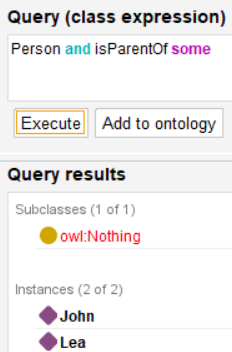
\includegraphics[width=\textwidth]{images/1.1 - tuto/q2.png}
        \caption{Persons who are Parents}
        \label{fig:image2}
    \end{minipage}
    \hfill
    \begin{minipage}[b]{0.25\textwidth}
        \centering
        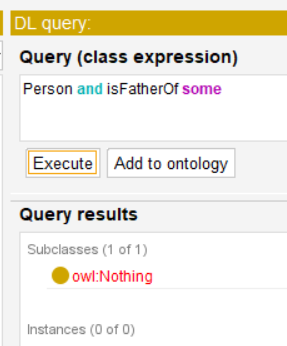
\includegraphics[width=\textwidth]{images/1.1 - tuto/q3.png}
        \caption{Persons who are Fathers : Issue there}
        \label{fig:image3}
    \end{minipage}
    
    \vspace{0.5cm} % Add vertical space between the rows
    
    \begin{minipage}[b]{0.4\textwidth}
        \centering
        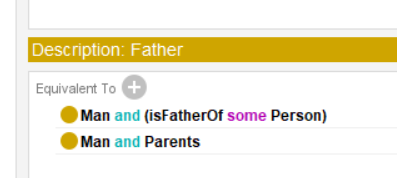
\includegraphics[width=\textwidth]{images/1.1 - tuto/q4 - adding an axiom to father .png}
        \caption{Adding two axiom to the Father Class}
        \label{fig:image4}
    \end{minipage}
    \hfill
    \begin{minipage}[b]{0.25\textwidth}
        \centering
        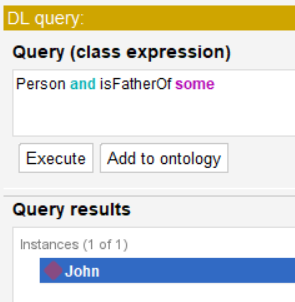
\includegraphics[width=\textwidth]{images/1.1 - tuto/q5 - now q3 works .png}
        \caption{This enabled the reasoner to infer that John is a Father}
        \label{fig:image5}
    \end{minipage}
    \label{fig:allimages}
\end{figure}

\subsection{Ontology of Ecosystem Interactions and Resource Consumption}


% We want to produce an ontology on an illustrative practical example aligned with the United Nations Sustainable Development Goals.

% \\
% We first choose a problem: 
% (for instance for sustainability, such as water consumption)

% \\ 
% Explain the design of the ontology (classes, data properties, object properties, class axioms, individuals...). Provide snapshots of the ontolgy (asserted and then inferred), and explain some queries2

To explore the logical relationships related to the consumption of natural resources and the environment, the theme chosen for the ontology was the model of an ecosystem, with a focus on the relationships and interactions among organisms (such as animals, plants, and microorganisms), their environments, and the resources they require.
\\

Overall, our model presents three main classes that interact with each other: the classes of \textbf{Organisms}, \textbf{Resources}, and \textbf{Habitats}. Organisms are further divided into three main subclasses: Animals, Plants, and Microorganisms. These organisms inhabit specific Environments and consume a set of natural resources provided by those environments.
\\

Additionally, important relationships can be inferred from this model, with the main ones being:


\begin{itemize}
    \item The relationship of coexistence, where two organisms cohabit the same environment without one being a predator of the other, or, when applied to microorganism, if they do not consume the same resource;

    \item Relationships involving the consumption of certain natural resources based on the characteristics of the organisms and the environment in which they live;

    \item Relationships concerning the food chain within the ecosystem, based on the type of food/energy source required by the organism along with characteristics of the environment.
    \\
\end{itemize}


The following image illustrates the relationship diagram that was implemented in the Protege software.

\begin{figure}[H]
    \centering
    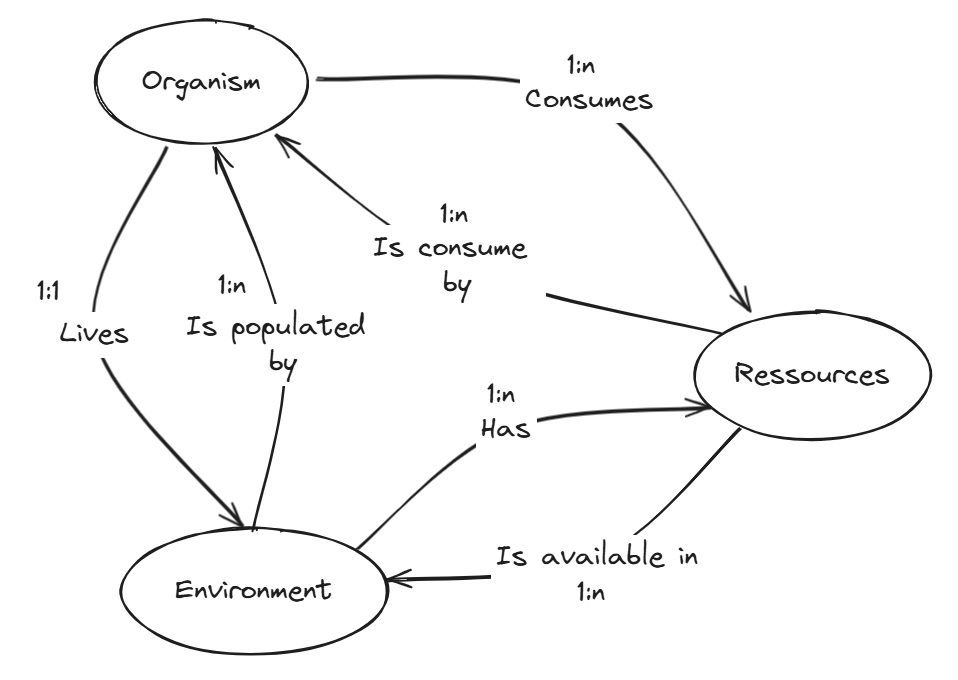
\includegraphics[width=0.7\linewidth]{diagram}
    \caption{Relationship diagram}
    \label{fig:diagram}
\end{figure}

In Figure \ref{fig:diagram}, there is a cardinality relation above the arrows. These relate \textit{m} individuals from the source category with \textit{n} individuals from the target category. For example, the "Consumes" relation going from Organism to Resource indicates that 1 individual can consume \textit{n} resources. Conversely, its symmetric relation, "Is consumed by," indicates that 1 resource can be consumed by \textit{n} organisms.


\section{Protege implementation}

The following describes the classes and subclasses used to create the ontology in Protege.
\\

\begin{itemize}
    \item \textbf{Classes} (that are subclasses of owl:Thing):
    \begin{itemize}
        \item Organism;

        \item Habitat;

        \item Resource.
        \\
    \end{itemize}

    \item \textbf{Subclasses}:
    \begin{itemize}
        \item Animal, Plant and Microorganism as subclasses of Organism (all mutually disjoint from each other);

        \item Herbivore and Carnivore as subclasses of Animals (they are both disjoint);

        \item Bryophytes and  Angiosperms as subclasses of Plants (all mutually disjoint from each other).
        \\
    \end{itemize} 
\end{itemize}

It is important to note that all classes and subclasses are mutually exclusive; therefore, no individual from one class can belong to another, and no individual from one subclass can belong to another subclass. The hierarchy of classes can be better observed in the figure below.

\begin{figure}[H]
    \centering
    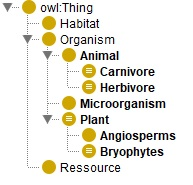
\includegraphics[width=0.35\linewidth]{images/ontology/classes.jpg}
    \caption{Class hierarchy}
    \label{fig:diagram}
\end{figure}


Regarding the Class properties, we have the following \textbf{Data properties}:
\\

    \begin{itemize}
        \item \textit{weight} with domain Animal and range xsd:decimal;

        \item \textit{has\_Fruits} with domain Angiosperms and range xsd:boolean;

        \item \textit{chemical\_formula} with domain Ressource and range xsd:string. We set this property to be unique, as it will be used as the identifier of the ressource;

        \item \textit{geographical\_coordinates} with domain Habitat and range xsd:string. It also has the unique property, and will be used as the identifier of the environment;

        \item \textit{scientific\_name} with domain Organism and range xsd:string. Again, it's unique and used as an indentifier for the organisms.
        \\

    \end{itemize}


The following two figures illustrate both the declaration of data properties and the method used to ensure the uniqueness of the \textit{scientific\_name}, for example.
\\

\begin{figure}[H]
    \centering
    \begin{minipage}{0.35\textwidth}
        \centering
        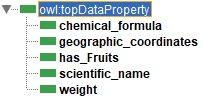
\includegraphics[width=\textwidth]{images/ontology/mini1.jpg}
        \caption{Data properties}
        \label{fig:figura1}
    \end{minipage}%
    \hspace{0.1\textwidth}
    \begin{minipage}{0.35\textwidth}
        \centering
        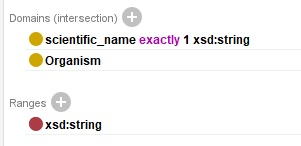
\includegraphics[width=\textwidth]{images/ontology/mini2.jpg}
        \caption{Unique property}
        \label{fig:figura2}
    \end{minipage}
\end{figure}

Finally, we have the following \textbf{Object properties}:
\\

    \begin{itemize}
        \item \textit{eat} with domain Animal and range Animal $\cup$ Plant;

        \item \textit{livesIn} with domain Organism and range Habitat;

        \item \textit{consumeTheResource} with domain Organism and range Resource;

        \item \textit{isEatenBy} with domain Organism and range Animal (is the inverse property \textit{eat});

        \item \textit{isOccupiedBy} with domain Habitat and range Organism (is the inverse of \textit{livesAt});

        \item \textit{hasTheResource} with domain Habitat and range Resource;

        \item \textit{isInTheEnvironment} with domain Resource and range Habitat (inverse of the property \textit{hasTheResource})

        \item \textit{coExistWith} with domain Organism and range Organism. This property is symmetric. In addition, this property is different if both organisms are animals/plants or if they are both microorganisms:
        \begin{enumerate}
            \item $A$ and $B$ are animals/plants: \textit{A} coexists with \textit{B} means that \textit{A} and \textit{B} lives at the same environment (livesIn(A) == livesIn(B)) \textbf{and} they do not share neither the relation \textit{A} isEatenBy \textit{B} nor \textit{B} isEatenBy \textit{A};

            \item $A$ and $B$ are both microorganisms: \textit{A} coexists with \textit{B} means that \textit{A} and \textit{B} lives at the same environment (livesIn(A) == livesIn(B)) \textbf{and} they do not consume the same resource through the relation consumeTheResource;
            \\
            
        \end{enumerate}
    \end{itemize}

The list of object properties in Protégé can be seen in the figure below.

\begin{figure}[H]
    \centering
    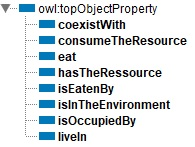
\includegraphics[width=0.35\linewidth]{images/ontology/obg_protp.jpg}
    \caption{Object properties}
    \label{fig:diagram}
\end{figure}

The inference rules were described using \textit{SWRL} (Semantic Web Rule Language), which allows for writing it in a practical and concise manner. Below, we provide a detailed description of all the inference rules related to object and data properties.
\\

We start by the following inference rule: if Organism $a$ eat Organism $b$, and Organism $a$ live in the Habit $env$, then $b$ should also live in $env$. This is described by:
\\

\begin{lstlisting}
eat(?a, ?b) ^ liveIn(?a, ?env) -> liveIn(?b, ?env)
\end{lstlisting}


The same way, if Organism $a$ coexists with Organism $b$, and $a$ live in the Habitat $env$, $b$ should also live in $env$.
\\

\begin{lstlisting}
coexistWith(?a, ?b) ^ liveIn(?a, ?env) -> liveIn(?b, ?env)
\end{lstlisting}

Now, regarding the plants, we can infer that a plant is an angiosperm if it has a fruit, which is a binary variable. Therefore, we have the following rule:
\\

\begin{lstlisting}
has_Fruits(?a, true) -> Angiosperms(?a)
\end{lstlisting}

From now on, we will focus on discussing the coexistence relationship, which is the most complex relation of the ontology. As previously described, according to our rules, a carnivorous animal will always coexist with another carnivorous animal as long as they inhabit the same environment. Additionally, we add the rule that animal $a$ must be different from $b$, as we do not want the relation to be reflexive. To ensure that they are both different, we require that their scientific names be different, using the syntax \textit{differentFrom}.
\\

\begin{lstlisting}
Carnivore(?a) ^ Carnivore(?b) ^ liveIn(?a, ?env) ^ liveIn(?b, ?env) ^ scientific_name(?a, ?name_a) ^ scientific_name(?b, ?name_b) ^ differentFrom(?name_a, ?name_b) -> coexistWith(?a, ?b)
\end{lstlisting}

We use the same logic to describe the coexistence for the herbivores, as follows:
\\

\begin{lstlisting}
Herbivore(?a) ^ Herbivore(?b) ^ liveIn(?a, ?env) ^ liveIn(?b, ?env) ^ scientific_name(?a, ?name_a) ^ scientific_name(?b, ?name_b) ^ differentFrom(?name_a, ?name_b) -> coexistWith(?a, ?b)
\end{lstlisting}

Also, carnivorous animals will always coexist with the plants that inhabit the same environment. In this case, it's enough to add the proposition \textit{differentFrom(?a, ?b)} because if $a$ is a Carnivore (by the previous proposition) and $b$ is a Plant (also stated earlier), they should be different because both classes are disjoint.
\\

\begin{lstlisting}
Carnivore(?a) ^ Plant(?b) ^ liveIn(?a, ?env) ^ liveIn(?b, ?env) ^ differentFrom(?a, ?b) -> coexistWith(?a, ?b)
\end{lstlisting}

Next, we have the case of coexistence between plants, which is similar to the herbivore's case:
\\


\begin{lstlisting}
Plant(?a) ^ Plant(?b) ^ liveIn(?a, ?env) ^ liveIn(?b, ?env) ^ scientific_name(?a, ?name_a) ^ scientific_name(?b, ?name_b) ^ differentFrom(?name_a, ?name_b) -> coexistWith(?a, ?b)
\end{lstlisting}

Finally, the coexistence between two microorganism happens when they both live in the same environment \textbf{and} do not consume the same resource. To guarantee that both resources are different, we use again their unique identifier, which is the \textit{chemical\_formula}:
\\

\begin{lstlisting}
Microorganism(?a) ^ Microorganism(?b) ^ consumeTheResource(?a, ?res_a) ^ consumeTheResource(?b, ?res_b) ^ liveIn(?a, ?env) ^ liveIn(?b, ?env) ^chemical_formula(?res_a, ?formula_a) ^ chemical_formula(?res_b, ?formula_b) ^ differentFrom(?formula_a, ?formula_b) ^ scientific_name(?a, ?name_a) ^ scientific_name(?b, ?name_b) ^ differentFrom(?name_a, ?name_b) -> coexistWith(?a, ?b)
\end{lstlisting}


\subsection{Inferences and Queries}
We now create some individuals with the classes and object properties stated in the section above to analyze the reasoner's ability to inter them. We give only a limited set of details to each individual, in the hopes that the reasoner could fill in the holes and show us intuitive relations we thought beforehand.

All the examples created for Plants, Microorganisms, Animals, and Resources are in Tables \ref{tab:plants},\ref{tab:micro}, \ref{tab:res}, and \ref{tab:animals}. We highlight the fact that some properties are clearly missing, like for Oxygen and Water, not clearly stated to be in Savanna. We also mention that the individual Habitat, Savanna, was not programmed with any properties, reason why it's not included in one of the tables.

 
\begin{table}[h!]
    \begin{center}
        \caption{Individuals for plants}
        \begin{tblr}{colspec={|c| c | c|}}
            \hline
            % \multicolumn{4}{|c|}{Plants} \\
            % \hline
            Name& Attributes &Properties\\
            \hline
            { \vspace{0.1in} \\ Acacia}   & {\\ Has fruits\\ Acacia dealbata}    &{Consumes water \\ Found in Savanna \\ Consumes CO2\\ Consumes O2}\\
            \hline
            {Apple} &   {Has fruits \\ Malus domestica}  & {Consumes water}   \\
            \hline
            Grass & & {Consumes CO2 \\ Consumes water}\\
            \hline
        \end{tblr}
        \label{tab:plants}
    \end{center}
\end{table}


 
\begin{table}[h!]
    \begin{center}
        \caption{Individuals for microorganisms}
        \begin{tblr}{colspec={|c| c | c|}}
            \hline
            % \multicolumn{4}{|c|}{Plants} \\
            % \hline
            Name& Attributes &Properties\\
            \hline
            { Bacteria}   & {Escherichia coli}    &{Consumes CO2}\\
            \hline
            {NitroBacteria} &   {Nitrobacter alkalicus}  & {Consumes N2}   \\
            \hline
        \end{tblr}
        \label{tab:micro}
    \end{center}
\end{table}
\newpage
\begin{table}[h!]
    \begin{center}
        \caption{Individuals for resources}
        \begin{tblr}{colspec={|c| c | c|}}
            \hline
            % \multicolumn{4}{|c|}{Plants} \\
            % \hline
            Name& Attributes &Properties\\
            \hline
            {  Carbon Dioxide}   & {CO2}    &{Is in Savanna}\\
            \hline
            {Nitrogen} &   {N2}  & {Is in Savanna}   \\
            \hline
            Oxygen & O2 &\\
            \hline
            Water & H2O &\\
            \hline
        \end{tblr}
        \label{tab:res}
    \end{center}
\end{table}

\begin{table}[h!]
    \begin{center}
        \caption{Individuals for animals}
        \begin{tblr}{colspec={|c| c | c|}}
            \hline
            Name& Attributes &Properties\\
            \hline
            { \\Cow}   & {Weight \\ Bos taurus}    &{Eats grass\\ Consumes water\\ Consumes O2}\\
            \hline
            {\\Giraffe} &   {Weight \\ Giraffa camelopardalis}  & {Eats Acacia\\ Consumes water \\ Consumes O2}\\
            \hline
            {\\Human} & {\\Weight} & {Eats Apple \\ Eats Cow\\ Not eaten by Lion\\ Consumes water\\ Consumes O2}\\
            \hline
            {\\ Lion}& {\\ Weight\\ Panthera leo}&{Eats Giraffe \\ Eats Zebra\\ Found in Savanna\\Consumes water\\ Not eaten by Human }\\
            \hline
            {\\ Zebra}&{\\ Weight \\ Equus quagga} & {Eat Apple\\ Consumes O2\\ Consumes water\\ Eats Grass}\\
            \hline
        \end{tblr}
        \label{tab:animals}
    \end{center}
\end{table}


We now run the reasoner, HermiT, and present some snapshots of the inferences found by it.

\newpage


\subsubsection{Plant Inferences}

We begin with the first two plants in our individual's collection: Acacia and Apple.

\begin{figure}[h!]
    \centering
    \begin{subfigure}[b]{0.8\linewidth}
      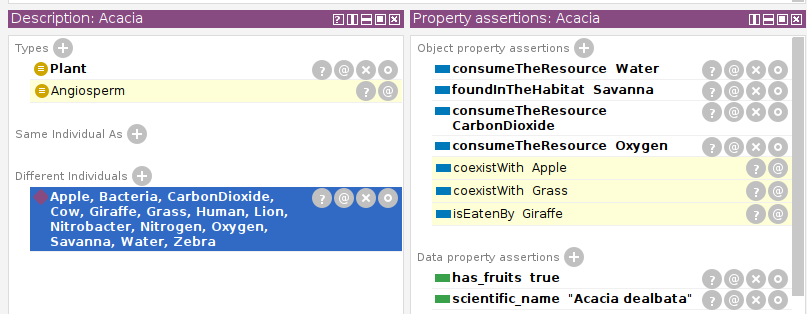
\includegraphics[width=\linewidth]{images/inferences/acacia_inf.png}
      \caption{Acacia's description on Protégé.}
    \end{subfigure}
    \begin{subfigure}[b]{0.8\linewidth}
      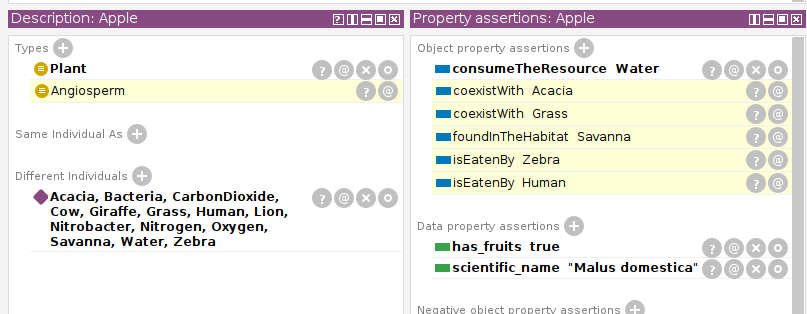
\includegraphics[width=\linewidth]{images/inferences/apple_inf.png}
      \caption{Apple's description on Protégé.}
    \end{subfigure}
    \caption{Inference showcase for both Acacia and Apple individuals of the Plant subclass.}
    \label{fig:acaciaapple_inf}
\end{figure}

  As we can see by \autoref{fig:acaciaapple_inf}, the reasoner is capable of inferring that both plants are Angiosperms, just by the presence of the fruit in their attributes. It's also able to infer their coexistence, between themselves and with Grass, Acacia's property of being eaten by Giraffe, Apple's localization in Savanna and the fact its consumed by both Humans and Zebras.

  In \autoref{fig:grass_inf} we see Grass' inferences for its coexistence with Apple and Apacia, its localization in Savanna, and the fact it's eaten by Zebras and Cows.

  \begin{figure}[h!]
    \centering
    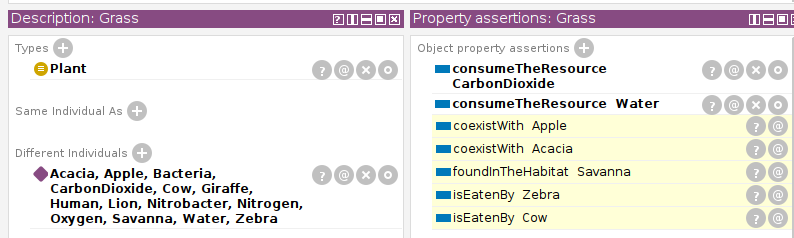
\includegraphics[width=0.8\linewidth]{images/inferences/grass_inf.png}
    \caption{Grass' description on Protégé.}
    \label{fig:grass_inf}
  \end{figure}

  \newpage
  \subsection{Microorganism Inferences}
  For the microorganisms, we check \autoref{fig:micro_inf}. Both of their localization was inferred to be Savannas, and also the fact they coexist, that could be deduced by the fact both consume different resources: Bacteria consumes $CO_{2}$, and NitroBacteria, $N_{2}$.

\begin{figure}[h!]
    \centering
    \begin{subfigure}[b]{0.8\linewidth}
      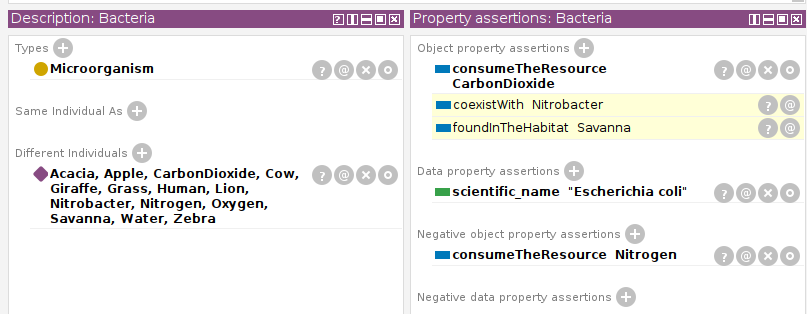
\includegraphics[width=\linewidth]{images/inferences/bac_inf.png}
      \caption{Bacteria's description on Protégé.}
    \end{subfigure}
    \begin{subfigure}[b]{0.8\linewidth}
      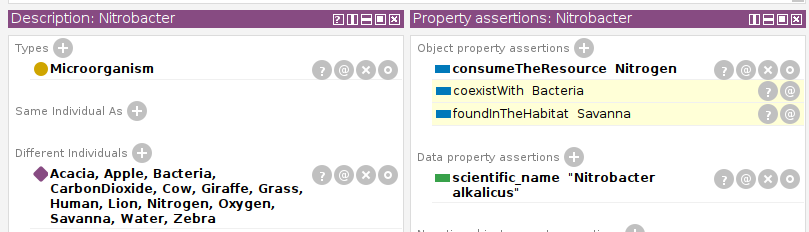
\includegraphics[width=\linewidth]{images/inferences/nitrobac_inf.png}
      \caption{NitroBacteria's description on Protégé.}
    \end{subfigure}
    \caption{Inference showcase for both Bacteria and NitroBacteria individuals of the Microorganism subclass.}
    \label{fig:micro_inf}
\end{figure}

\subsection{Resources inferences}

In \autoref{fig:co2n2_inf}, we see the inferences for Carbon Dioxide($CO_{2}$) and Nitrogen($N_{2}$), which most involves they're being consumed by the right individuals, without explicit mention of those in their properties. For Oxygen($O_{2}$) and water($H_{2}O$), similar inferences are showcased in \autoref{fig:h2oco2_inf}, but now involve a way bigger number of \textit{isConsumedBy} properties, and also the fact they're in Savanna.

\begin{figure}[h!]
    \centering
    \begin{subfigure}[b]{0.8\linewidth}
      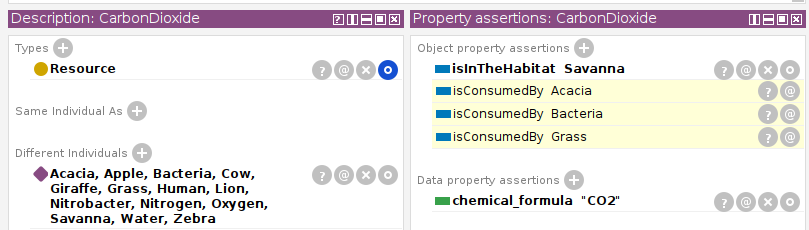
\includegraphics[width=\linewidth]{images/inferences/co2_inf.png}
      \caption{Carbon Dioxide's description on Protégé.}
    \end{subfigure}
    \begin{subfigure}[b]{0.8\linewidth}
      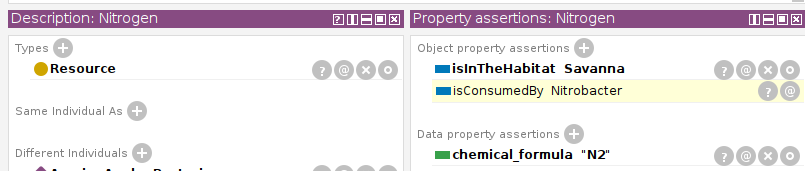
\includegraphics[width=\linewidth]{images/inferences/nitrogen_inf.png}
      \caption{Nitrogen's description on Protégé.}
    \end{subfigure}
    \caption{Inference showcase for both Carbon Dioxide and Nitrogen individuals of the Resource subclass.}
    \label{fig:co2n2_inf}
\end{figure}



\begin{figure}[h!]
    \centering
    \begin{subfigure}[b]{0.8\linewidth}
      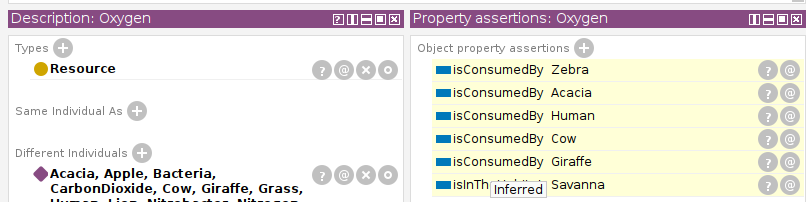
\includegraphics[width=\linewidth]{images/inferences/oxygen_inf.png}
      \caption{Oxygen's description on Protégé.}
    \end{subfigure}
    \begin{subfigure}[b]{0.8\linewidth}
      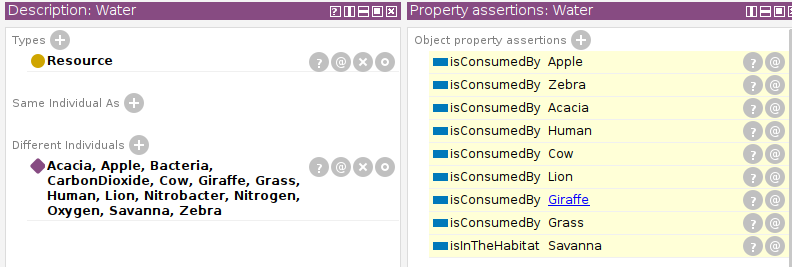
\includegraphics[width=\linewidth]{images/inferences/water_inf.png}
      \caption{Water's description on Protégé.}
    \end{subfigure}
    \caption{Inference showcase for both Oxygen and Water of the Resource subclass.}
    \label{fig:h2oco2_inf}
\end{figure}

\newpage

\subsection{Animals inferences}

We begin by the showcase of our Herbivores inferences, in \autoref{fig:cowzebra_inf}. Aside from the correct coexistence between each other and their predators, the reasoner is also capable of classifying each one of them as \textit{Herbivore}, from the fact they only eat Plants.

\begin{figure}[h!]
    \centering
    \begin{subfigure}[b]{0.8\linewidth}
      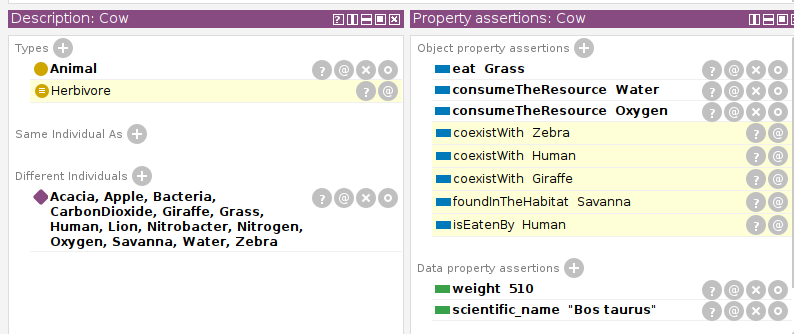
\includegraphics[width=\linewidth]{images/inferences/cow_inf.png}
      \caption{Cow's description on Protégé.}
    \end{subfigure}
    \begin{subfigure}[b]{0.8\linewidth}
      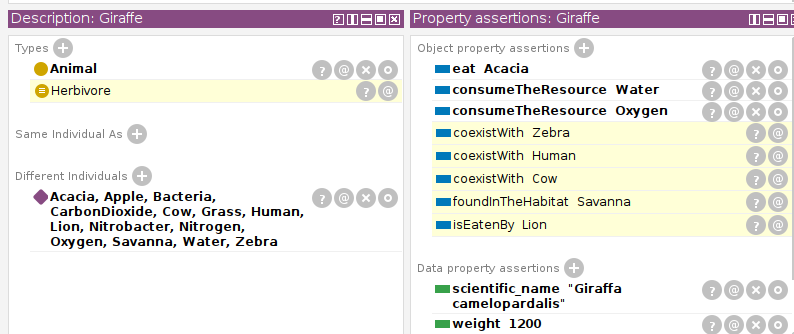
\includegraphics[width=\linewidth]{images/inferences/giraffe_inf.png}
      \caption{Giraffe's description on Protégé.}
    \end{subfigure}
    \begin{subfigure}[b]{0.8\linewidth}
        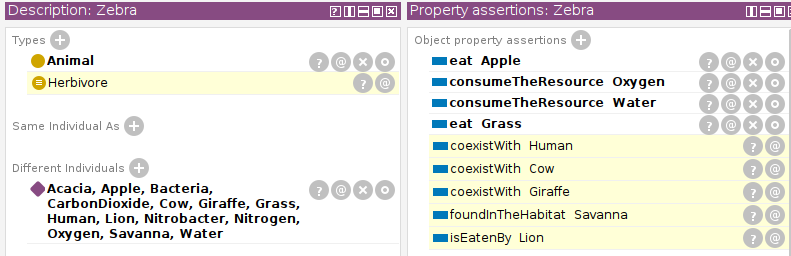
\includegraphics[width=\linewidth]{images/inferences/zebra_inf.png}
        \caption{Zebra's description on Protégé.}
      \end{subfigure}
    \caption{Inference showcase for Cow, Giraffe, and Zebra individuals of the Animal subclass.}
    \label{fig:cowzebra_inf}
\end{figure}

\newpage

Human's and Lion's inferences can be found in \autoref{fig:humanlion_inf}. First we highlight the inference that Lion is a Carnivore from the fact he only eats meat. Second, Human's classification as a Omnivore for the diversity in the resources and Animals it consumes.

\begin{figure}[h!]
    \centering
    \begin{subfigure}[b]{0.8\linewidth}
      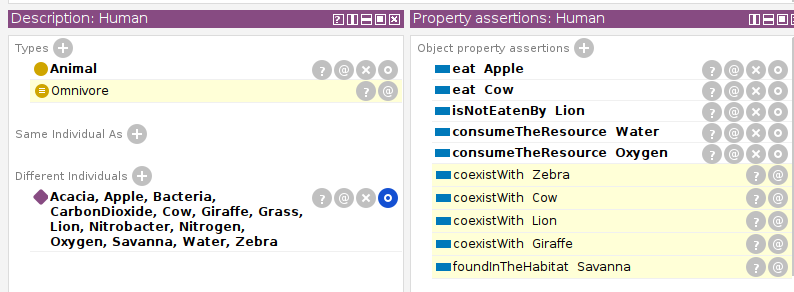
\includegraphics[width=\linewidth]{images/inferences/human_inf.png}
      \caption{Human's description on Protégé.}
    \end{subfigure}
    \begin{subfigure}[b]{0.8\linewidth}
      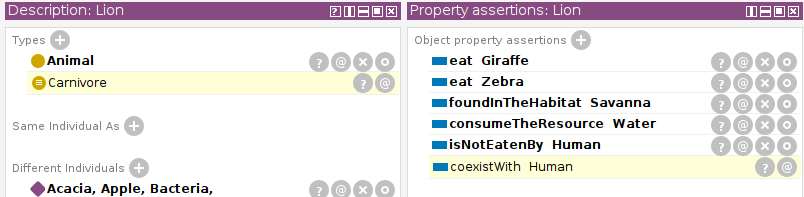
\includegraphics[width=\linewidth]{images/inferences/lion_inf.png}
      \caption{Lion's description on Protégé.}
    \end{subfigure}
    
    \caption{Inference showcase for Human and Lion individuals of the Animal subclass.}
    \label{fig:humanlion_inf}
\end{figure}


\end{document}